\chapter{Vorlesung}
\section{Priority-Queue mittels Fibonacci-Heaps (Fortsetzung)}
\subsection{Lemma}
Für jeden Knoten $x$ in einem Fibonacci-Heap gilt, dass die Zahl aller Knoten im Unterbaum von $x$ mindestens $\Phi^k$ beträgt, wobei $k = \grad(x)$.
\subsection{Beweis}
\begin{wrapfigure}{L}{0.5\linewidth}
	\centering
	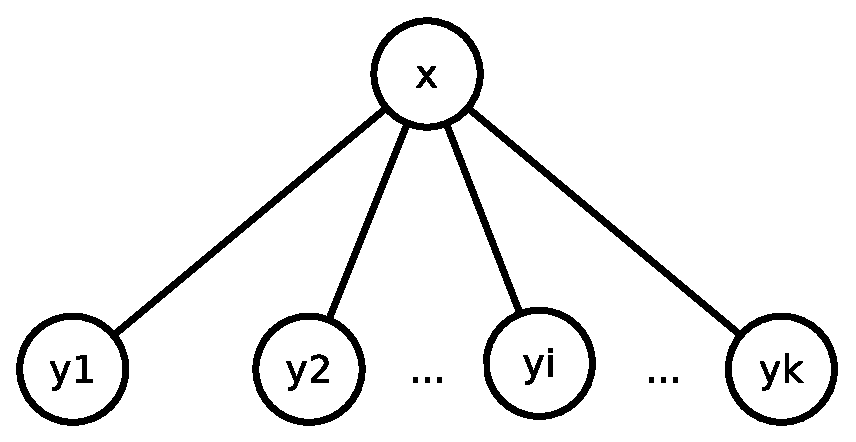
\includegraphics[width=\linewidth]{22/Grafik/Diagramm1}
	\caption{Schaubild zum Beweis}
	\label{fig:beweis}
\end{wrapfigure}
Seien $y_1, y_2,\ldots,y_k$ die aktuellen Kindknoten von $x$, nummeriert in der Reihenfolge, wie sie (letztmalig) Kindknoten von $x$ geworden sind. Zum Zeitpunk, zu dem $y_i$ Kindknoten von $x$ geworden ist, existieren bereits die $i-1$ Kindknoten $y_1, y_2,\ldots,y_{i-1}$. $\Rightarrow\grad(x)\geq i-1$\\ 
$y_i$ kann nur Kind von $x$ werden, wenn $x$ und $y_i$ gleichen Grad haben. $\Rightarrow\grad(y_i)\geq i-1$\\
Da $y_i$ im Folgenden höchstens einen Kindknoten verlieren kann, gilt:
\[ \grad(y_i) \geq i-2 \]
Sei $S_k$ die Mindestanzahl von Knoten in einem Unterbaum eines Knoten $x$ vom Grad $k$
\[ S_k \geq 1+1+\sum_{i=2}^{k} S_{i-2} \]
Wir zeigen
\[ S_k\overset{(2)}{\geq} f_{k+2}\footnote{$k-2$-te Fibonacci Zahl}\overset{(1)}{\geq}\Phi^k \]

\begin{wraptable}[-5]{R}{0.3\linewidth}
	\centering
	\begin{tabular}{ccccccc}
		$f_0$&$f_1$&$f_2$&$f_3$&$f_4$&$f_5$&$\ldots$\\
		$0$&$1$&$1$&$2$&$3$&$5$& 
	\end{tabular}
\end{wraptable}
\paragraph{(1)}
\[ f_{k+2}\geq \Phi^k \]
\[ k=0~:~ f_2=1\geq\Phi^0=1 \]
\[ k=1~:~ f_3=2\geq\Phi^1=1,6181\ldots \]
\[ f_{k+2} = f_{k+1}+f_k \geq \Phi^{k-1}+\Phi^{k-2}=\footnote{$\Phi^2=\Phi+1$} \Phi^{k-2}(\Phi+1)=\Phi^{k-2}\cdot\Phi^2=\Phi^k \]
\paragraph{(2)}
\[ S_k \geq f_{k+2} \text{?}\]
\[ S_k\geq 2+\sum_{i=2}^{k}S_{i-2} \]
\[ k=0~:~S_0\geq f_2=1~~\checkmark \]
\[ k=1~:~S_1\geq f_3=2~~\checkmark \]
\[ S_k \geq 2+\sum_{i=2}^{k}f_i\text{, da wegen Induktions-Annahme }S_{i-2}\geq f_{(i-2+2)}=f_i \text{ für }i<k \]
\paragraph{Zu zeigen:}
\[ 2 + \sum_{i=2}^{k}f_i \geq f_{k+2} \]
\paragraph{Es gilt:}
\[ 1+\sum_{i=1}^{k}f_i=f_{k+2} \]
\[ k=0~:~1=f_2~\checkmark \]
\[ k=1~:~1+f_1=f_3=2~\checkmark \]
\[ 1+\sum_{i=1}^{k+1} = (1+\sum_{i=1}^{k}f_i)+f_{k+1} = f_{k+2}+f_{k+1}=f_{k+3} \]
\begin{flushright}
	q.e.d.
\end{flushright}

Aus dem Lemma folgt, dass in einem Fibonacci-Heap für $n$\footnote{$\Phi^k\leq n$} Elemente zu keinem Zeitpunkt ein Knoten vom Grad $\log_\phi n = k$ auftauchen kann. Insbesondere ist die Wurzelliste nach einer Konsolidierung auch nur $\log_\Phi n$ lang, weil dort nur Knoten unterschiedlichen Grades auftauchen. 


\pagebreak

\subsection{Satz}
Mit einem Fibonacci-Heap lassen sich die Operationen \texttt{insert}, \texttt{deleteMin} und \texttt{decreaseKey} mit folgenden amortisierten Kosten realisieren:\\
\begin{tabular}{ll}
	\texttt{insert}&$\mathcal{O}(1)$\\
	\texttt{deletemin}&$\mathcal{O}(\log n)$\\
	\texttt{decreaseKey}&$\mathcal{O}(1)$
\end{tabular} 

\subsection{Beweis}
Wir verwenden die Bankkonto-Methode zur amortisierten Analyse nach folgendem Schema:\\
Jeder Knoten in der Wurzelliste wird mit einer RE\footnote{Rechen Einheit} bespart und jeder markierte Knoten der einen Kindknoten verloren hat wird mit 2 RE bespart.
\paragraph{Bemerkung}
Wurzelknoten tragen keine Markierung, obwohl sie eventuell Kindknoten verloren haben.\\

Wir zeigen nun, dass die oben genannten Kosten für die einzelnen Operationen ausreichen, damit im gesamten Verlauf das Kontoführungsschema, ohne Schulden machen zu müssen, aufrecht erhalten werden kann.\\
\begin{description}
	\item[\texttt{insert}] Einfügen in Wurzelliste $+1$RE Investition $\in\mathcal{O}(1)$\\
	\item[\texttt{deleteMin}] Alle Kindknoten des gelöschten Knotens wandern in die Wurzelliste.\\ Dafür müssen wir $\log_\Phi n$ viele RE investieren. Die Konkatenation der doppelt verketteten Listen kostet nur konstante Zeit. Der ganze Konsolidierungsprozess kann bezahlt werden durch die RE auf den Wurzelknoten. Die anschließende Minimumsuche kostet nur $\mathcal{O}(\log n)$, weil die Wurzelliste höchstens $\log_\Phi n$ viele Elemente hat.
	\item[\texttt{decreaseKey}] $ $
	\paragraph{Behauptung} Es genügen 4 RE pro Operation\\
	Vorgehensweise:
	\begin{itemize}
		\item 1RE für die Aufnahme eines abgelösten Knotens in die Wurzelliste
		\item 2RE für die Markierung des Vaterknotens
		\item 1RE für "`sonstige"' konstante Kosten(Pointeraktualisierungen).
	\end{itemize}
	Ein Vaterknoten, der schon markiert ist, hat aufgrund der Gültigkeit der Bankkontoführung schon 2RE und bekommt vom abgelösten Kindknoten noch 2 RE. Damit hat er 4RE für seine eigene Ablösung zur Verfügung. Dieses Schema lässt sich also fortsetzen und die Kosten einer Ablösekaskade lassen sich damit decken. %siehe http://www.duden.de/rechtschreibung/aufgrund_Praeposition
\end{description}
\begin{flushright}
	q.e.d.
\end{flushright}